\documentclass{beamer}

%% Juego de caracteres usado en el archivo fuente: UTF-8
\usepackage{ucs}
\usepackage[utf8x]{inputenc}
\usepackage{graphicx}
\usepackage{eurosym}
\uselanguage{spanish}
%Para la identación del español
\usepackage[spanish]{babel}



% There are many different themes available for Beamer. A comprehensive
% list with examples is given here:
% http://deic.uab.es/~iblanes/beamer_gallery/index_by_theme.html
% You can uncomment the themes below if you would like to use a different
% one:
%\usetheme{AnnArbor}
%\usetheme{Antibes}
%\usetheme{Bergen}
%\usetheme{Berkeley}
%\usetheme{Berlin}
%\usetheme{Boadilla}
%\usetheme{boxes}
%\usetheme{CambridgeUS}
%\usetheme{Copenhagen}
%\usetheme{Darmstadt}
%\usetheme{default}
%\usetheme{Frankfurt}
%\usetheme{Goettingen}
%\usetheme{Hannover}
%\usetheme{Ilmenau}
%\usetheme{JuanLesPins}
%\usetheme{Luebeck}
\usetheme{Madrid}
%\usetheme{Malmoe}
%\usetheme{Marburg}
%\usetheme{Montpellier}
%\usetheme{PaloAlto}
%\usetheme{Pittsburgh}
%\usetheme{Rochester}
%\usetheme{Singapore}
%\usetheme{Szeged}
%\usetheme{Warsaw}


\title{Cableado estructurado}

% A subtitle is optional and this may be deleted
%\subtitle{Optional Subtitle}

\author{Redes de Computadores}


% - Give the names in the same order as the appear in the paper.
% - Use the \inst{?} command only if the authors have different
%   affiliation.

%\institute[Escuela Superior de Ingeniería] % (optional, but mostly needed)
%{
%  \inst{1}%
%  Department of Computer Science\\
%  University of Somewhere
%  \and
%  \inst{2}%
%  Department of Theoretical Philosophy\\
%  University of Elsewhere}
% - Use the \inst command only if there are several affiliations.
% - Keep it simple, no one is interested in your street address.

\date{GrupoLaboratorio\_2}
% - Either use conference name or its abbreviation.
% - Not really informative to the audience, more for people (including
%   yourself) who are reading the slides online

%\subject{Theoretical Computer Science}
% This is only inserted into the PDF information catalog. Can be left
% out. 

% If you have a file called "university-logo-filename.xxx", where xxx
% is a graphic format that can be processed by latex or pdflatex,
% resp., then you can add a logo as follows:

% pgfdeclareimage[height=0.5cm]{university-logo}{university-logo-filename}
% \logo{\pgfuseimage{university-logo}}

% Delete this, if you do not want the table of contents to pop up at
% the beginning of each subsection:
%\AtBeginSubsection[]
%{
%  \begin{frame}<beamer>{Índice}
%    \tableofcontents[currentsection,currentsubsection]
%  \end{frame}
%}

% Let's get started
\begin{document}

\begin{frame}
	\titlepage
\end{frame}

\begin{frame}{Trabajo realizado por:}
	  \begin{itemize}
	  \item{Borja Caro Macho}
	  \item{Alejandro Cuesta Contreras}
	  \item{Manuel Fernández Rosado}
	  \item{Francisco Javier Jiménez Vázquez}
	  \item{Arantzazu Otal Alberro}
	  \item{Francisco Javier Pérez Sánchez}
	  \item{Juan Pedro Rodríguez Gracia}
	  \item{Jesús Rodríguez Heras}
	  \item{Gabriel Fernando Sánchez Reina}
	  \item{José Antonio Torres Leal}
	  \end{itemize}
\end{frame}



\begin{frame}{Índice}
  \tableofcontents
  % You might wish to add the option [pausesections]
\end{frame}

% Section and subsections will appear in the presentation overview
% and table of contents.
\section{Planos de cableado horizontal}
\subsection{Planta baja}

\begin{frame}{Planos de cableado horizontal: Planta baja}
%	Para Ordenar puntos utilizar el itemsize de abajo
%  \begin{itemize}
%  \item {
%    Punto 1.
%  }
%  \item {
%    Punto 2.
%  }
%  \end{itemize}
\begin{center}
	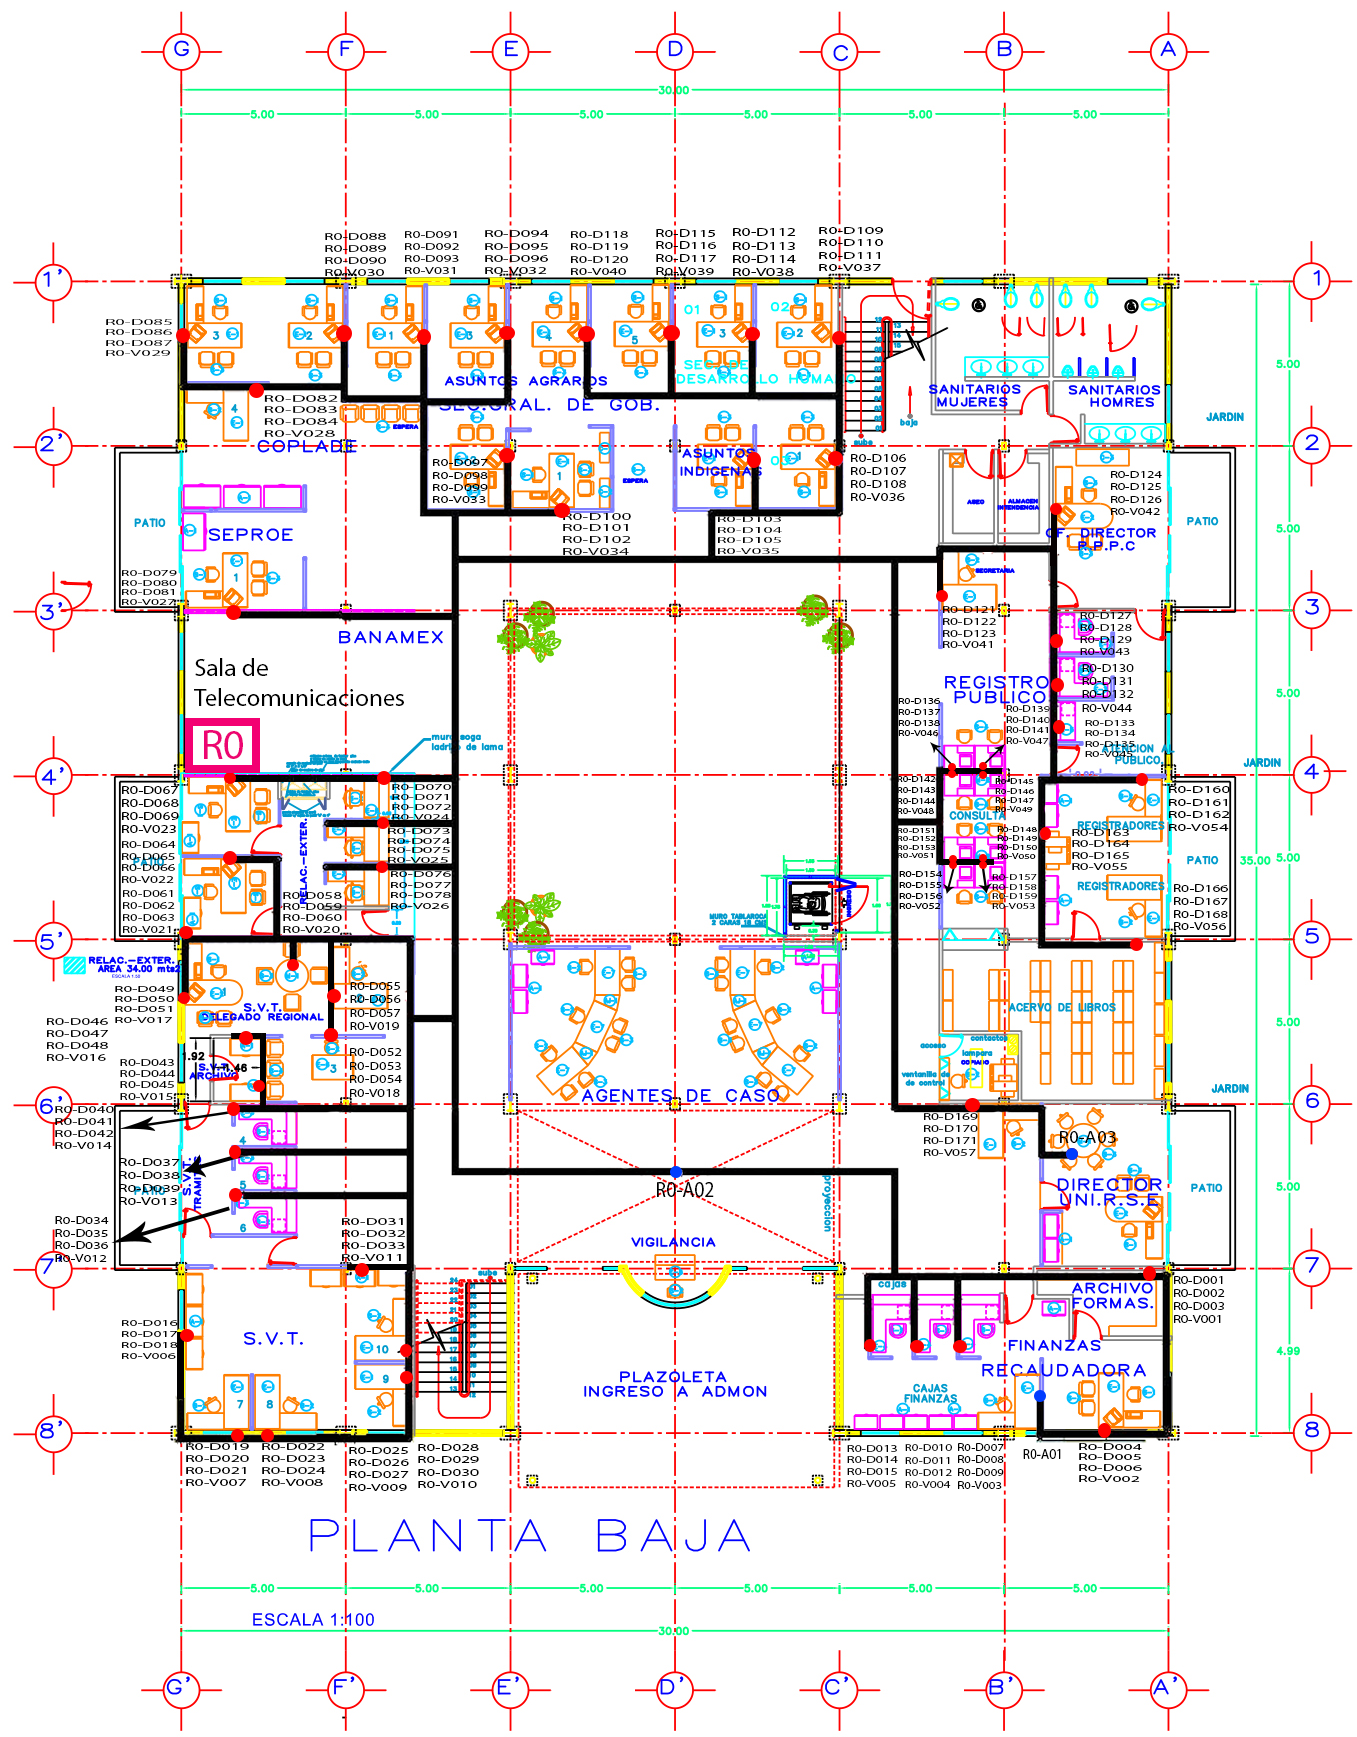
\includegraphics[scale=0.54]{CHPB.png}
\end{center}

\end{frame}


\subsection{Planta alta}
% You can reveal the parts of a slide one at a time
% with the \pause command:
\begin{frame}{Planos de cableado horizontal: Planta alta}
\begin{center}
	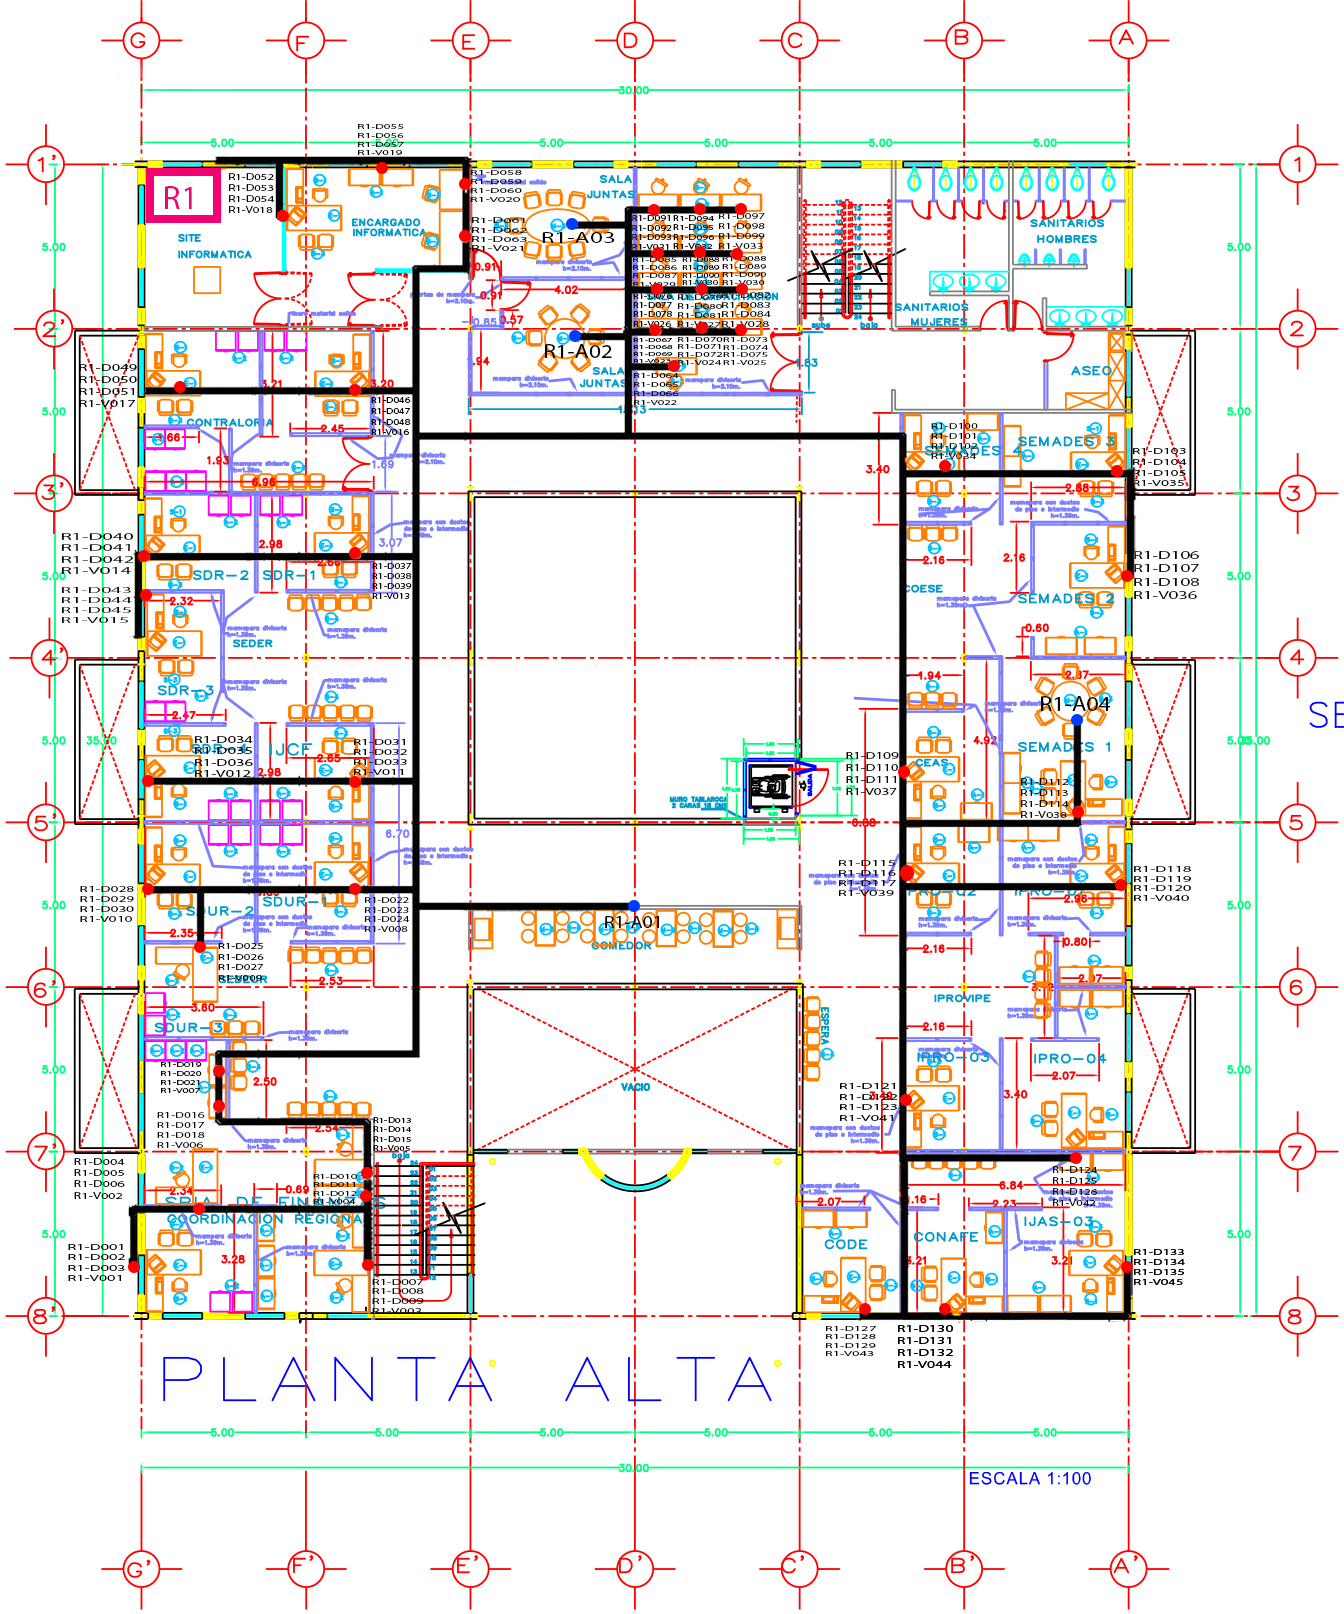
\includegraphics[scale=0.57]{CHPA.png}
\end{center}
\end{frame}


\subsection{Etiquetado}
% You can reveal the parts of a slide one at a time
% with the \pause command:
\begin{frame}{Detalle del etiquetado}
\begin{center}
	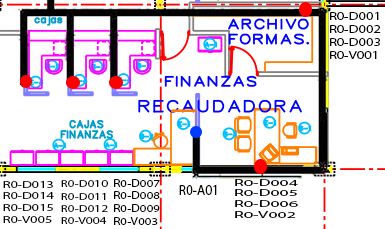
\includegraphics[scale=2.5]{DetallePB.png}
\end{center}
\end{frame}


\section{Plano de conexión}
\begin{frame}{Plano de conexión}
\begin{center}
	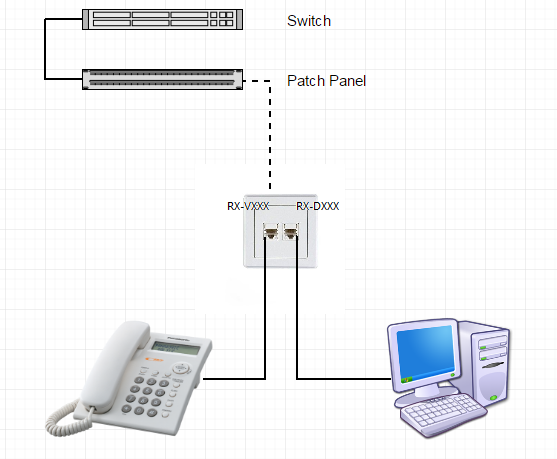
\includegraphics[scale=0.6]{area_trabajo.png}
\end{center}
\end{frame}



\section{Plano de cableado vertical}

\begin{frame}{Plano de cableado vertical}
\begin{center}
	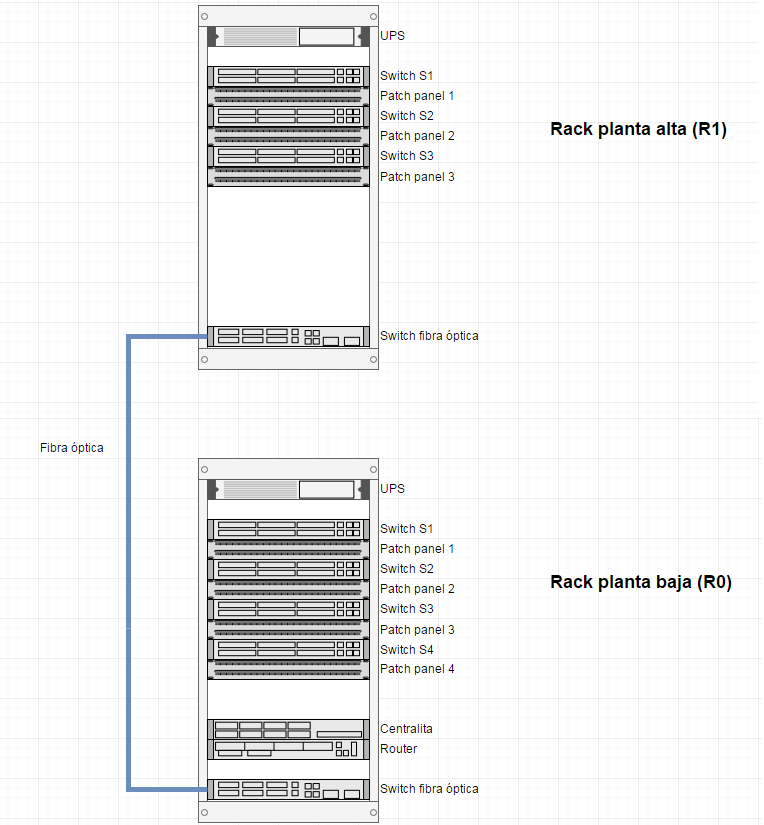
\includegraphics[scale=0.34]{CV.png}
\end{center}	
\end{frame}


\section{Distribuidores}
\subsection{Rack 0}
\begin{frame}{Distribuidores. Rack 0}
\begin{center}
	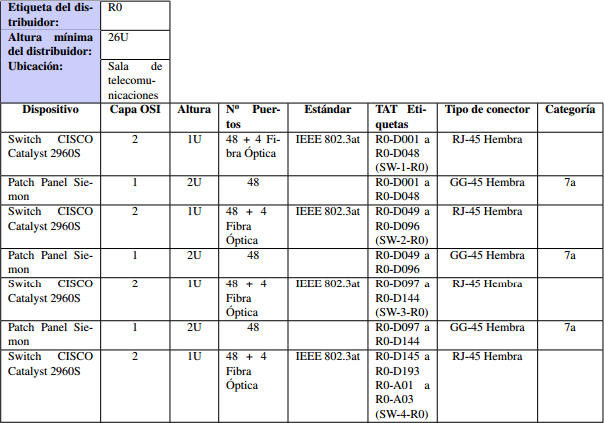
\includegraphics[scale=0.65]{r0-1.png}
\end{center}
\end{frame}

\begin{frame}{Distribuidores. Rack 0}
\begin{center}
	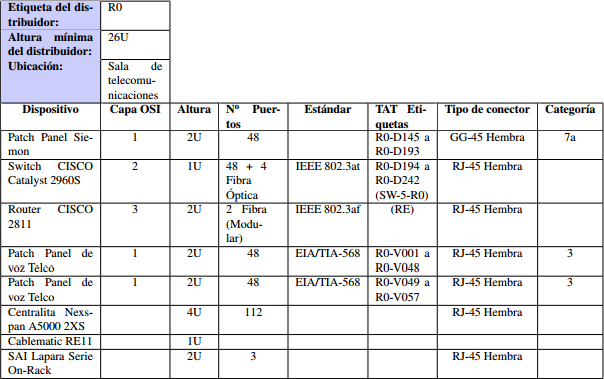
\includegraphics[scale=0.62]{r0-2.png}
\end{center}
\end{frame}

\subsection{Rack 1}
\begin{frame}{Distribuidores. Rack 1}
\begin{center}
	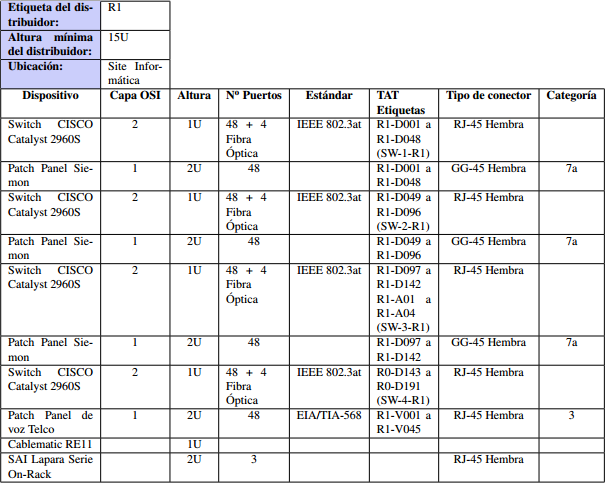
\includegraphics[scale=0.6]{r1.png}
\end{center}
\end{frame}

\section{Preguntas}
\begin{frame}{Preguntas}
\begin{center}
	
\includegraphics[scale=0.58]{Preguntas.png}\\
	¿Alguna pregunta?
\end{center}
\end{frame}


\end{document}



